\documentclass[11pt]{beamer}
\usetheme{Warsaw}
\usepackage[utf8]{inputenc}
\usepackage[T1]{fontenc}
\usepackage{amsmath}
\usepackage{amsfonts}
\usepackage{amssymb}
\usepackage{graphicx}
\author{Fernando Del Fedele}
\title{Crecimiento y caracterización de
láminas delgadas con memoria de
forma de alta temperatura Ni-Ti-Zr
mediante sputtering.}
%\setbeamercovered{transparent} 
%\setbeamertemplate{navigation symbols}{} 
%\logo{} 
%\institute{} 
%\date{} 
%\subject{} 
\begin{document}

\begin{frame}
\titlepage
\end{frame}

\begin{frame}{Contenido}
\tableofcontents
\end{frame}

\section{Introducción}
\subsection{Objetivo}
\subsection{Materiales con memoria de forma}
\begin{frame}{Materiales con memoria de forma}
Las aleaciones con memoria de forma, de aquí en adelante nombradas como \textbf{SMA} (del inglés, \textbf{S}hape \textbf{M}emory \textbf{A}lloys) son aleaciones que pueden recuperar su forma original al ser calentadas luego de haber sufrido una deformación aparentemente plástica
Entre sus propiedades, se encuentran:
\begin{itemize}
	\item Superelasticidad
	\item Alta capacidad de amortiguamiento
	\item Alta relación entre la potencia entregada y su peso
\end{itemize}
\end{frame}
\subsection{Materiales con memoria de forma de alta temperatura}
\begin{frame}
Las aplicaciones actuales de los SMA están limitadas por debajo de los $100^\circ C$. Los materiales con memoria de forma de alta temperatura, abreviados como \textbf{HTSMA} (del inglés, \textbf{H}igh \textbf{T}emperature \textbf{S}hape \textbf{M}emory \textbf{A}lloys) son aquellos en los cuales la transformación martensítica sucede a $T > 100^\circ C$.

Lo más común a es a $NiTi$ agregarle $Pd$ o $Pt$ en detrimento del $Ti$, pero recientemente se encontró que $Hf$ o $Zr$ tienen efectos aún mayores en la temperatura a menor costo relativo.
\end{frame}
\subsection{Transformación martensítica}
\begin{frame}{Transformación martensítica}
La causa del efecto de memoria de forma es la transformación martensítica.
Sus propiedades son
\begin{itemize}
	\item Transformación de estado sólido
	\item Primer orden
	\item Sin difusión atómica
	\item Desplazamiento de los átomos del orden de 1 \AA
	\item Los átomos mantienen relación con sus vecinos cercanos
\end{itemize}
\end{frame}
\begin{frame}
La fase de menor temperatura, B19' pasa a la fase B2, que tiene mayor simetría al aumentar la temperatura. La fase recordada es aquella que está en la fase B2. Agregar imagen
\end{frame}
\begin{frame}{Termodinámica de la transformación}

\end{frame}
\section{Técnicas experimentales}
\subsection{Deposición por magnetrón sputtering}
\begin{frame}{Deposición por magnetrón sputtering}
\begin{figure}[H]
	\centering
	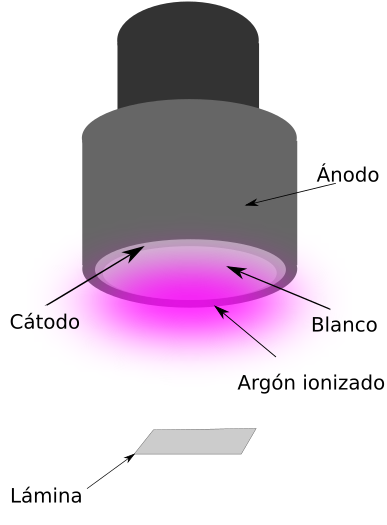
\includegraphics[scale=0.1]{img/SchemaDeposition.png}
	\caption{Magnetrones empleados durante las deposiciones.}
	\label{magnetrones}
\end{figure}
\begin{figure}[H]
	\centering
	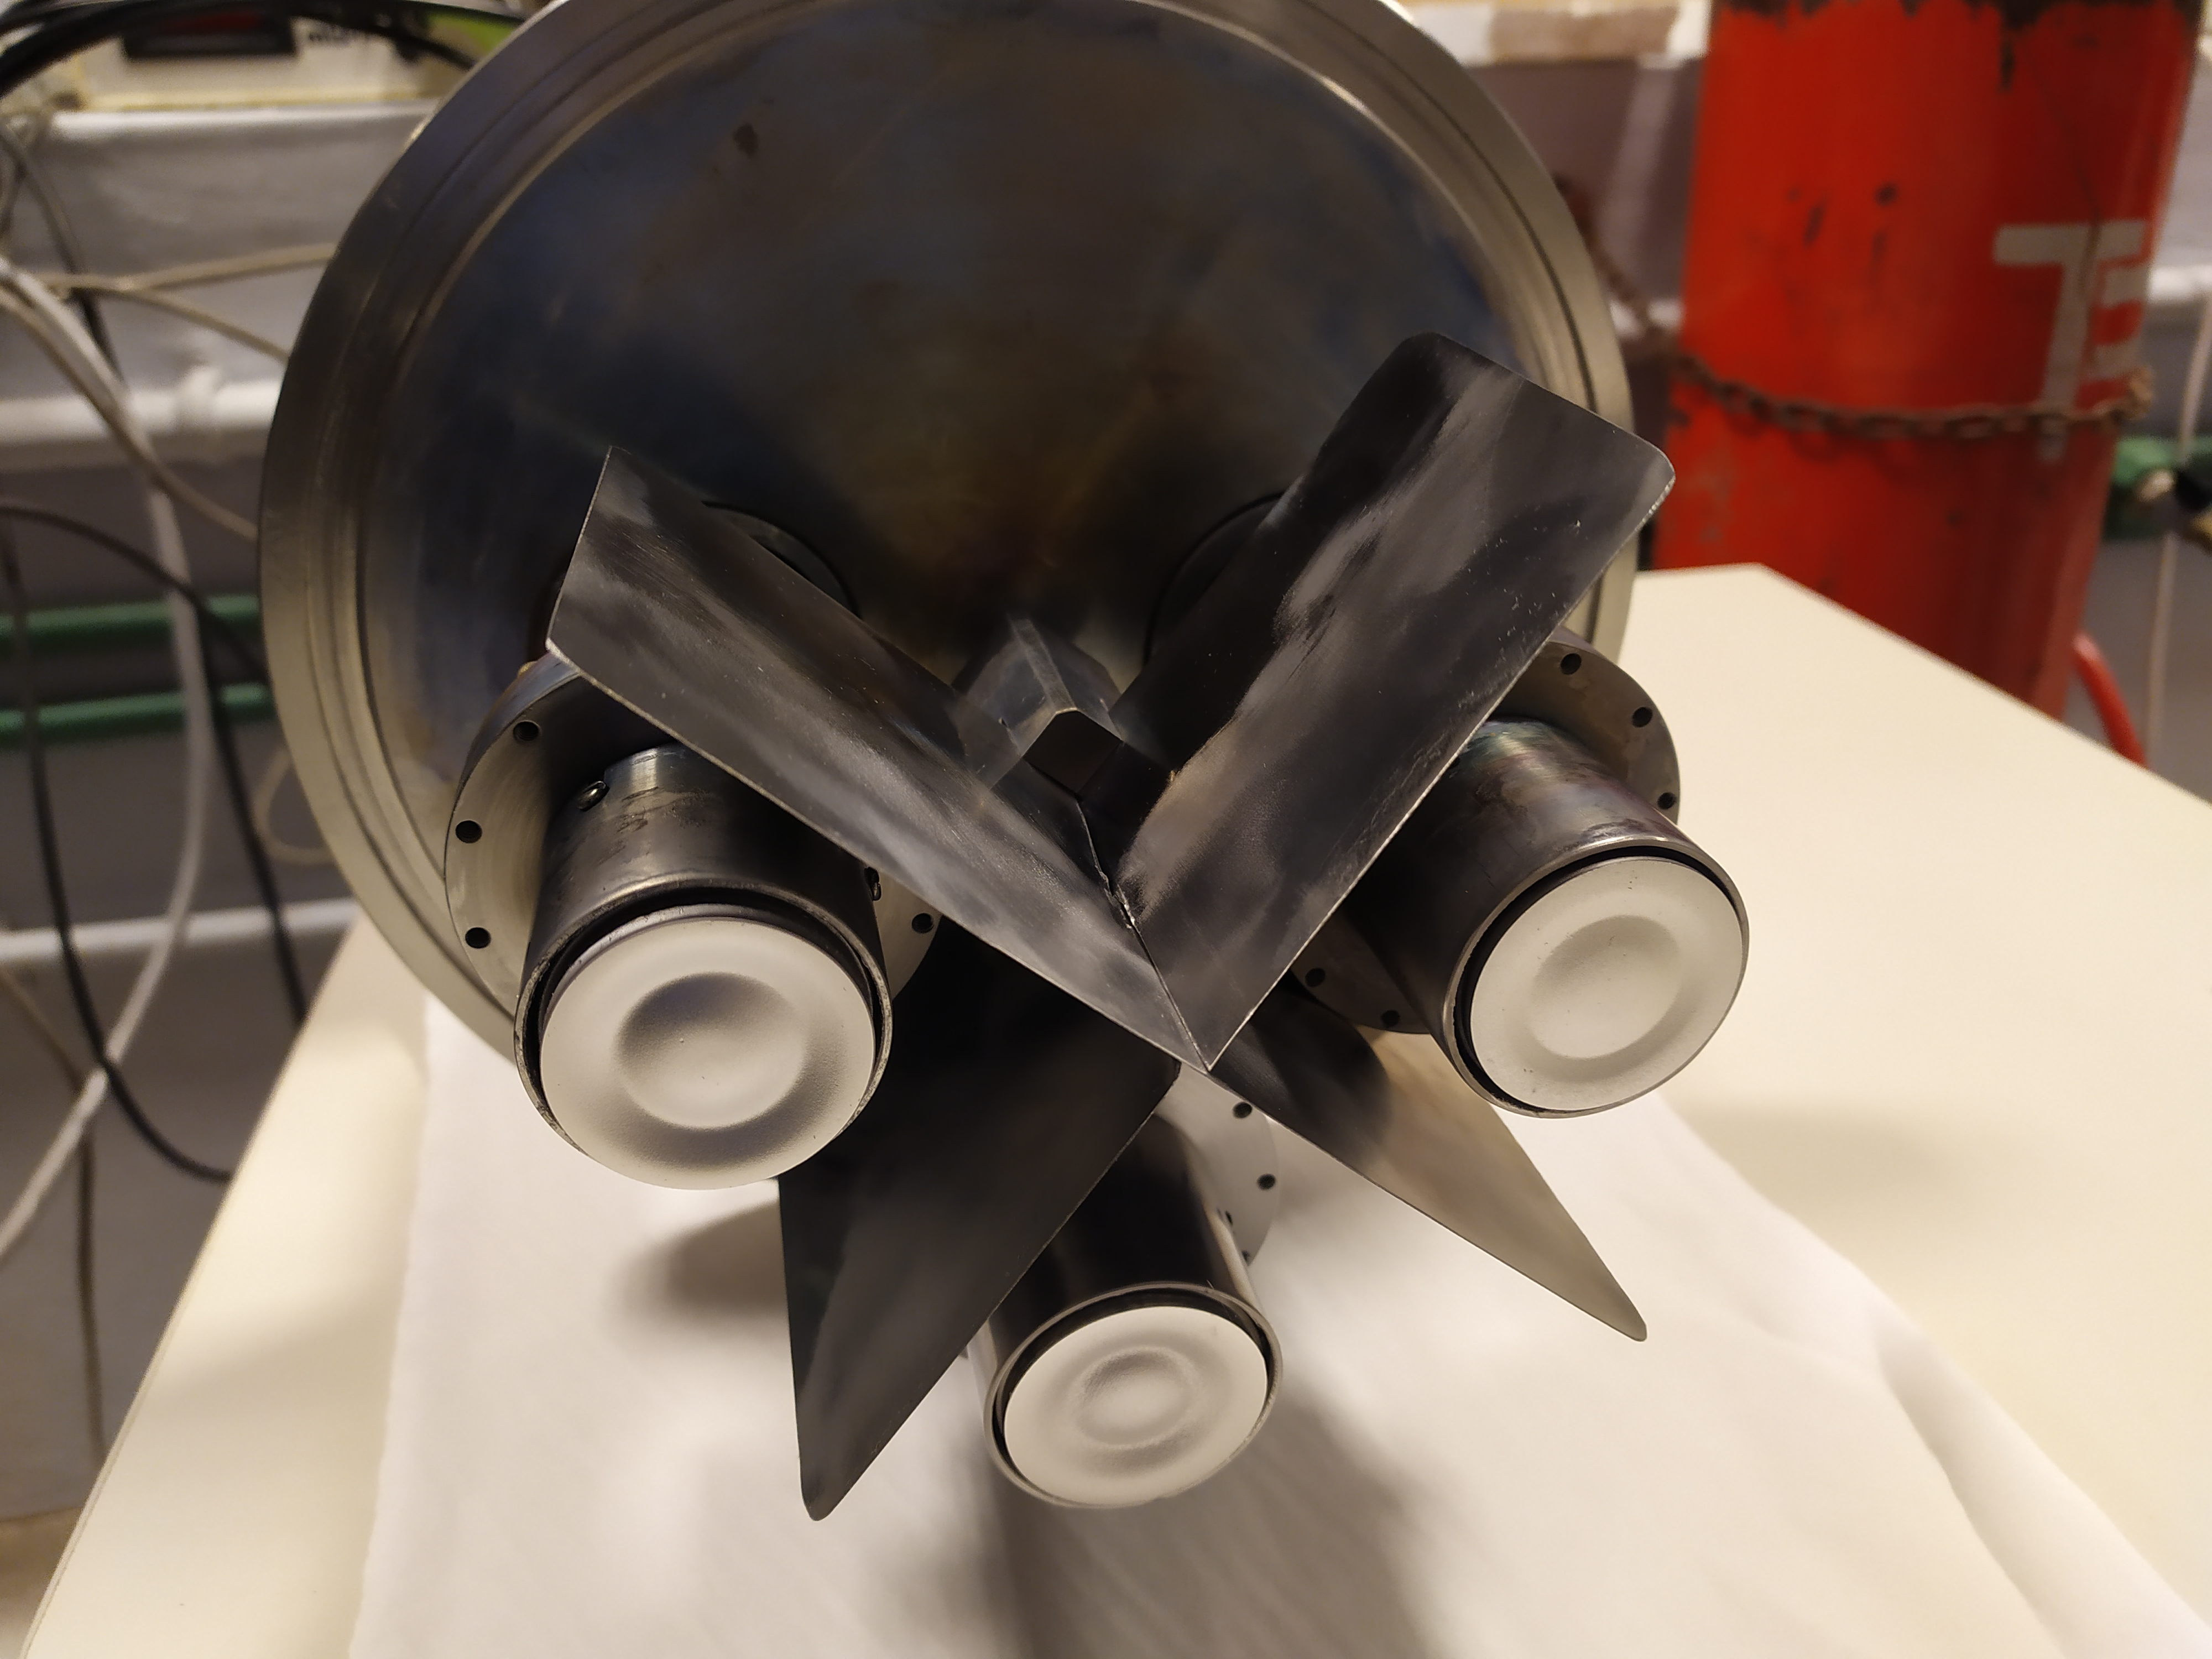
\includegraphics[scale=0.1]{img/magnetrones.jpg}
	\caption{Magnetrones empleados durante las deposiciones.}
	\label{magnetrones}
\end{figure}
\end{frame}
\subsection{Microscopía electrónica de barrido}
\subsection{Difracción por rayos X}
\subsection{Microscopía electrónica de transmisión}
\subsection{Calorimetría diferencial de barrido}
\subsection{Resistividad por el método de cuatro puntas}
\section{Resultados obtenidos}
\section{Discusión}
\section{Conclusión}

\end{document}